% !TeX program = pdflatex
% Minimally-Congested Travel Time Prediction from Sparse Open Data
% Authors: Geoff Boeing and Yuquan Zhou
% Web: https://geoffboeing.com/
% Repo: https://github.com/gboeing/travel-time-prediction

\newcommand{\myname}{Geoff Boeing and Yuquan Zhou}
\newcommand{\myemail}{boeing@usc.edu}
\newcommand{\myaffiliation}{University of Southern California}
\newcommand{\paperdate}{2025}
\newcommand{\papertitle}{Minimally-Congested Travel Time Prediction from Sparse Open Data}
\newcommand{\papercitation}{Boeing, G. and Y. Zhou. \paperdate. \papertitle. Under review at \emph{Journal Name}.}
\newcommand{\paperkeywords}{Urban Planning, Transportation, Data Science}

\RequirePackage[l2tabu,orthodox]{nag} % warn if using any obsolete or outdated commands
\documentclass[12pt,letterpaper]{article} % document style

% import encoding and font packages for pdflatex, in order
\usepackage[T1]{fontenc} % output T1 font encoding (8-bit) so accented characters are a single glyph
\usepackage[utf8]{inputenc} % allow input of utf-8 encoded characters
\usepackage{ebgaramond} % document's serif font
\usepackage{tgheros} % document's sans serif font

% import language, regionalization, microtype, and setspace in order
\usepackage[strict,autostyle]{csquotes} % smart and nestable quote marks
\usepackage[USenglish]{babel} % automatically regionalize hyphens, quote marks, etc
\usepackage{microtype} % improves text appearance with kerning, etc
\usepackage{setspace} % configure spacing between lines
\usepackage{mathtools} % use package math tool
% import everything else
\usepackage{abstract} % allow full-page title/abstract in twocolumn mode
\usepackage{amsmath}
\usepackage{authblk} % footnote-style author/affiliation info
\usepackage{booktabs} % better looking tables
\usepackage{caption} % custom figure/table caption styles
\usepackage{datetime} % enable formatting of date output
\usepackage[final]{draftwatermark} % watermark paper as a draft
\usepackage{endnotes} % enable endnotes
\usepackage{geometry} % configure page dimensions and margins
\usepackage{graphicx} % better inclusion of graphics
\usepackage{hyperref} % hypertext in document
\usepackage{natbib} % author-year citations w/ bibtex, including textual and parenthetical
\usepackage{rotating} % rotate wide tables or figures on a page to make them landscape
\usepackage{titlesec} % custom section and subsection heading
\usepackage{url} % make nice line-breakble urls
\usepackage{makecell}

% print only the month and year when using \today
\newdateformat{monthyeardate}{\monthname[\THEMONTH] \THEYEAR}

% location of figure files, via graphicx package
\graphicspath{{./figures/}}

% configure the page layout, via geometry package
\geometry{
    paper=letterpaper, % paper size
    top=3.8cm, % margin sizes
    bottom=3.8cm,
    left=4cm,
    right=4cm}
\setstretch{1} % line spacing
\clubpenalty=10000 % prevent orphans
\widowpenalty=10000 % prevent widows

% set section/subsection headings as the sans serif font, via titlesec package
\titleformat{\section}{\normalfont\sffamily\large\bfseries\color{black}}{\thesection.}{0.3em}{}
\titleformat{\subsection}{\normalfont\sffamily\small\bfseries\color{black}}{\thesubsection.}{0.3em}{}
\titleformat{\subsubsection}{\normalfont\sffamily\small\color{black}}{\thesubsubsection.}{0.3em}{}

% make figure/table captions sans-serif small font
\captionsetup{font={footnotesize,sf},labelfont=bf,labelsep=period}

% configure pdf metadata and link handling, via hyperref package
\hypersetup{
    pdfauthor={\myname},
    pdftitle={\papertitle},
    pdfsubject={\papertitle},
    pdfkeywords={\paperkeywords},
    pdffitwindow=true, % window fit to page when opened
    breaklinks=true, % break links that overflow horizontally
    colorlinks=false, % remove link color
    pdfborder={0 0 0} % remove link border
}

\begin{document}

\title{\papertitle}
\author[]{Redacted for review}%{\myname}
\affil[]{Redacted for review}%{\myaffiliation}
\date{}%{\paperdate}

\maketitle

\begin{abstract}

Travel time prediction is central to accessibility analyses, sustainable transportation infrastructure provision, and active transportation interventions. However, calculating accurate travel times, especially for driving, requires either extensive technical capacities and bespoke data, or sources like the Google Maps API that quickly becomes prohibitively expensive to analyze thousands or millions of trips necessary for metropolitan-scale planning. These obstacles make it difficult for researchers, practitioners, and community advocates to develop an evidence base for more sustainable transportation and equitable accessibility. This article develops a free, open-source minimally-congested driving time prediction model with minimal cost, data, and computational requirements. It trains and tests this model using the Los Angeles, California urban area as a case study by calculating naïve travel times then developing a predictive random forest regression model of Google Maps' \enquote{gold standard} travel times using those naïve times plus turns and traffic controls along the naïve routes. Validation reveals that this method yields accurate, free, and simple travel time predictions.

\end{abstract}

\section{Introduction}

Travel time prediction underpins many transport planning processes and research problems. It is key to understanding urban accessibility, transport mode and route choice, and location decisions. Predicting congested travel times (i.e., when traffic congestion impedes flows) requires large volumes of real-time data on traffic conditions. Such data are proprietary, expensive, and beyond the reach of many planning practitioners and scholars. This is usually not a problem for well-resourced organizations with highly-skilled labor. However, technical expertise, complex data and software requirements, and high costs pose insurmountable obstacles for many urban planning researchers, practitioners, and community advocates.

Although typical \enquote{naïve} travel time prediction methods (which minimize travel distance or street segment traversal time) provide easy solutions, they ignore delays from turns and traffic controls and thus usually under-predict real-world driving travel time. However, minimally-congested travel time prediction offers a middle ground of more-accurate predictions than naïve travel times do---yet much lower data and computing requirements than traffic-aware and congested travel time prediction.

To address this need for a middle ground, this article contributes a simple, accurate, and free method of minimally-congested driving travel time prediction. Our results show a substantial improvement over traditional, naïve methods of travel time prediction common in the urban planning literature. As we shall show in this article, across the Los Angeles urban area, our average trip's travel time prediction differs on average from Google's \enquote{gold standard} prediction by only 0.38 seconds. In contrast, simple---but common---naïve travel time prediction minimizing max-speed edge traversal times under-predicts Google's travel times by 182.71 seconds, on average.

The rest of this article is organized as follows. First it reviews the state of the art in travel time prediction and then considers the less-sophisticated methods that are standard in the current planning literature. Next it describes our data sources, models, and validation techniques. Then it presents our findings, highlighting both the feasibility and quality of our predictions in relation to simple naïve predictions or difficult expensive predictions. Finally, it concludes with a discussion of implications for research and practice.

\section{Background}

Modern travel time prediction techniques tend to fall into one of two camps: (1) sophisticated, accurate, but difficult to execute; or (2) naïve, less-accurate, but simple to execute. The former is the state-of-the-art and has been the subject of much work in the recent computer science and engineering literatures. The latter tends to appear often in urban planning research and practice. Here we summarize the recent advances and current standards in these fields.

\subsection{State-of-the-Art Travel Time Prediction}

Recent studies in the computer science and engineering literatures propose a variety of prediction techniques with heavy computing and data requirements. They usually measure their prediction accuracy by mean absolute percentage error (MAPE), defined in Equation~\ref{eq:mape}:

\begin{equation}
\label{eq:mape}
\text{MAPE} = \frac{100}{n} \sum^{n}_{i=1} \left|\frac{t_i - \hat{t_i}}{t_i}\right|
\end{equation}

where $n$ is the total number of trips, $t_i$ is trip $i$'s observed travel time, and $\hat{t_i}$ is trip $i$'s predicted travel time. Lower MAPEs indicate higher accuracy.  These studies usually yield MAPEs within roughly 10\% of observed driving times. Some researchers use alternative measures of accuracy, such as the percentage of over- or under-prediction \citep{jenelius2013travel}, the absolute mismeasurement in minutes \citep{chiabaut2021traffic}, or degrees of predictability \citep{li2019travel}.

These advanced travel time prediction models require massive data inputs as they are usually trained on millions or billions of disaggregate empirical travel time records. For example, \citet{hou2018network} use 1.5 billion GPS-based travel time records in deep learning models to predict travel time in 13 road segments in St. Louis, yielding a MAPE of 6.8\%. Using more than 100,000 trips from Windows phone GPS data, \citet{woodard2017predicting}'s technique achieves a MAPE of 10.1\% when predicting travel times. \citet{pamula2023estimation} use three months of video sensing data at a 5-minute temporal resolution in a deep learning model to predict travel times in Poland, yielding a 6.8\% MAPE.\@ Other studies use graph neural network models to predict travel times. For example, \citet{wang2023dynamic} use data from 100,000 Chinese ride-hailing trips in graph neural network and recurrent neural network models, yielding a MAPE of 15.4\%. \citet{vankdoth2023deep} achieve 3--4\% MAPEs using Q-Traffic and TaxiBJ data from Beijing and Chengdu in deep learning and graph neural network models.

Many of these studies focus on predicting travel times only for a specific street segment. For instance, \citet{sharmila2019svm} achieve a 10\% MAPE using GPS data in a support vector machine/particle filter model to predict travel times along specific arterials in Mumbai. \citet{chen2016multi}'s agent-based model uses data from GPS-equipped vehicles at 1-minute intervals across 123 days to achieve a MAPE under 9\% on a 95-mile freeway section in Virginia. Based on empirical travel time from GPS traces, road geometric features, and weather information, \citet{qiu2021machine} predict travel times using decision trees, random forests, extreme gradient boosting, and long short-term memory neural networks on the I-485 freeway in Charlotte, North Carolina, yielding MAPEs between 6--17\%.

As we have seen, these studies train or validate their models with a wide variety of bespoke data sources often collected from GPS devices or proprietary sources. The Google Maps API offers another common source. Though a black-box, many researchers use Google's travel times as the \enquote{gold standard} predictions of real-world travel times, given its ubiquity and accuracy and the challenges of otherwise directly obtaining sufficient empirical travel data \citep[e.g.,][]{goudarzi2018travel,stanojevic2019mapreuse,ludwig2023traffic}.

\subsection{Path Solving in Planning Research}

Central to all of the preceding travel time prediction research is the concept of \textit{path solving}: identifying the shortest path between an origin and destination in a spatial network model. In this case, the shortest path is defined as the path that minimizes travel time and could be realized methodologically in multiple ways. In the planning literature, studies variously minimize euclidean distance, network distance, network edge traversal time, free-flow travel time, or congested travel time. We discuss their trade-offs in this section.

The actual path solving methods used in urban planning research and practice tend to differ substantially from the state of the art travel time prediction in the engineering and computer science literatures. The preceding section's models require extensive technical capacity, instrumentation, and data. In general, the planning literature's implementations of path solving tend to be simpler to execute, but potentially naïve and less-accurate. For example, many accessibility studies employ merely a (very) rough proxy for travel time by minimizing euclidean distance traveled instead \citep[e.g.,][]{macfarlane2021modeling,pearsall2020locating}. This offers the substantial benefit of simplicity (no network model, travel time data, or routing algorithms are needed) but offers a poor estimate of access in terms of travel time.

Other studies improve on this by instead solving shortest paths by minimizing network distance traveled. These studies often use data and tools from Esri, OpenStreetMap, or the US Census Bureau to measure network distances between origins and destinations \citep[e.g.,][]{mckenzie2020urban, jiao2021measuring, nicoletti2023disadvantaged, logan2019evaluating, tsou2005accessibility}. This offers the benefit of more-realistic distances between origins and destinations, but does not account for travel speeds. Other studies refine this by incorporating speed limit data into the network model to solve shortest paths by traversal time \citep{kuai2017examining,williams2020parks,he2020evaluating,salonen2013modelling,scott2008role,neutens2010equity,wang2013planning}. Traversal time is similar to---but distinct from---uncongested travel time. The former merely minimizes the sum of the ratio of street segment length and speed limit, whereas the latter accounts for stops, signals, and turns. Some researchers sidestep the challenges of needing a network model and travel speed data by using secondary traffic analysis zone (TAZ) travel time data aggregated by metropolitan planning agencies \citep[e.g.,][]{grengs2010intermetropolitan,yan2021toward,levine2012does}. These data offer simplicity and real-world empricism, but their coarse-grained zone-to-zone aggregation obfuscates accurate point-to-point travel time predictions.

Finally, many planning scholars rely instead on the Google Maps API to obtain accurate origin-destination travel times and shortest paths \citep[e.g.,][]{fielbaum2021assessment,costa2021spatial, swayne2021integrating,hu2020estimating,cuervo2022dynamic,chen2020communities,hwang2024measuring}. As mentioned previously, Google travel times represent something of a \enquote{gold standard} in the literature, but come with drawbacks: the algorithms are closed-source and---for large batches of queries, such as for simulating metropolitan-scale trip taking---it can become prohibitively expensive and require many API queries. Nevertheless, evidence shows Google travel times offer a good approximation of real-world travel times \citep{lin2021impact,fu2023comparative,alsobky2020estimating,wang2011estimating}.

\subsection{Open Problem}

In summary, planning researchers today predict travel distances and times with a range of relatively simple techniques that minimize euclidean distance, network distance, street segment traversal time, TAZ-to-TAZ travel times, or Google travel times (for relatively few trips to keep costs down). These techniques are generally inexpensive and easy to implement. In contrast, today's state-of-the-art techniques in the computer science and engineering literatures require expensive data collection, private data, or much more complicated algorithms that planners are rarely trained to implement. In other words, it is expensive and challenging for the average planner to reproduce these state-of-the-art methods.

A better way would be to seek a middle ground between expensive, complicated, point-to-point empirical travel times and overly-simple naïve predictions. Such free empirical travel time predictions may not reflect congested travel times (which vary drastically throughout the day and week), but would provide a good prediction of minimally-congested travel times. This middle-ground method should meet three criteria. First, it should only use free software and free data, avoiding expensive and massive Google travel time queries or bespoke GPS data collection. Second, it should be a simple and accessible method for urban planners without advanced technical skills. Third, it should provide a substantial improvement in accuracy or spatial resolution over naïve predictions such as minimizing Euclidean distance, network distance, street edge traversal time, and exsiting TAZ-to-TAZ travel times, and approach the accuracy of the state-of-art models. Meeting these three criteria, a middle ground should be inexpensive, easy-to-use, and reasonably accurate.

\section{Methods}

This article proposes a new generalizable method to solve this problem. In short, it collects a small free amount of data from the Google Maps API plus free open data to train a local model to predict accurate minimally-congested travel times using relatively simple standard tools and techniques. Figure~\ref{fig:workflow} shows a detailed workflow.

\begin{figure*}[hbt!]
    \centering
    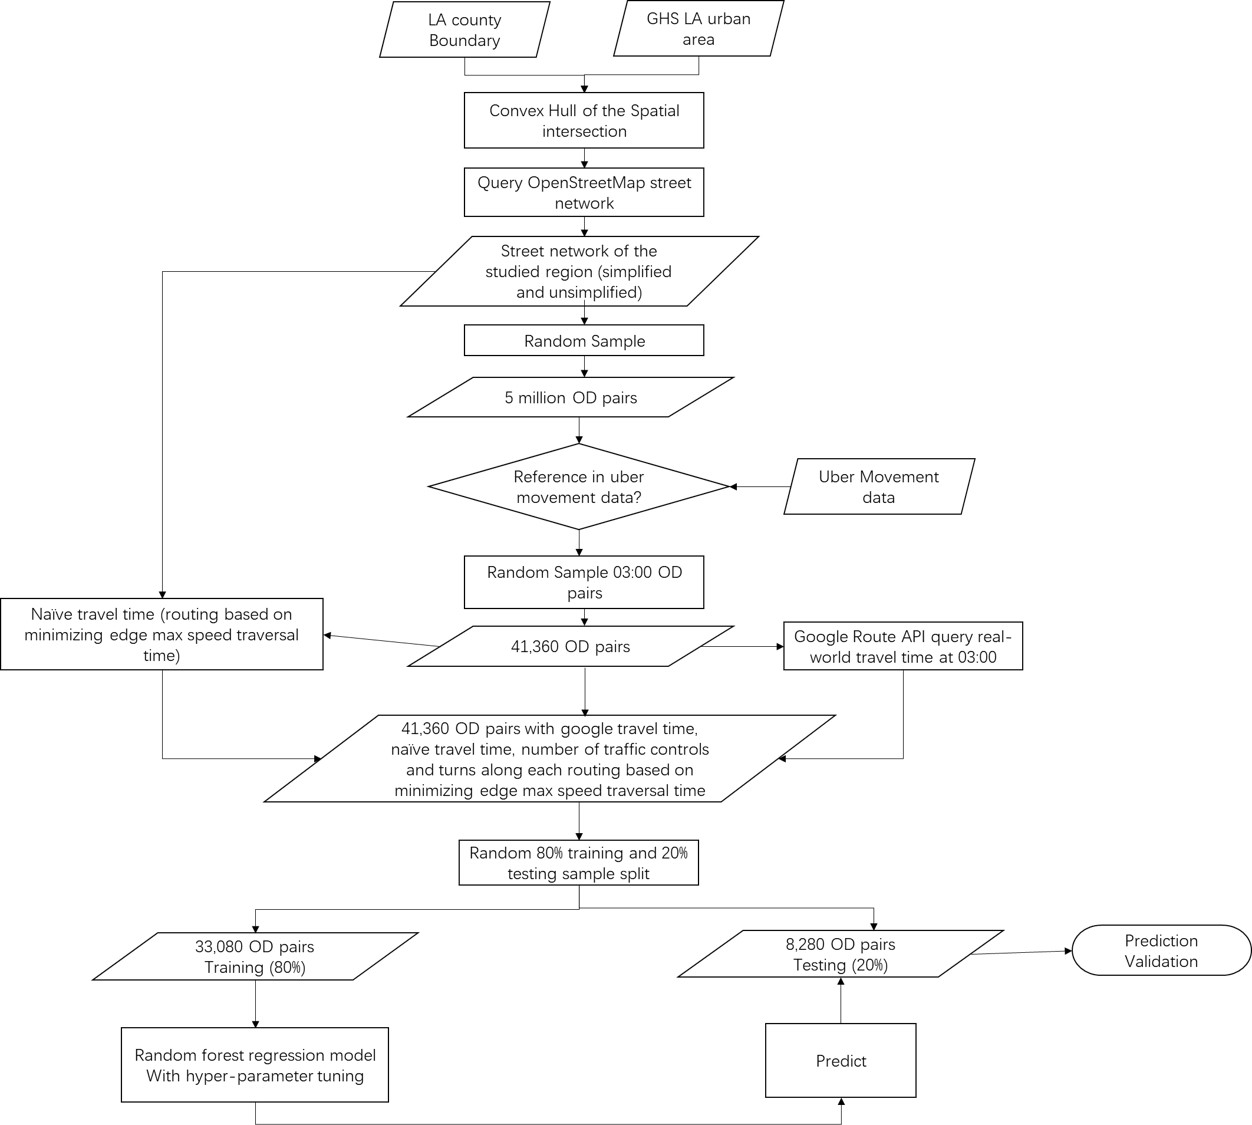
\includegraphics[width=1.0\textwidth]{fig_workflow.jpg}
    \caption{Detailed model workflow.}\label{fig:workflow}
\end{figure*}

\begin{table*}[hbt!]
    \centering
    \caption{Traffic control elements in the network model, as identified by OSM tags.}\label{tab:node_count}
    \begin{tabular}{lr}
        \toprule
        Traffic control element    & Node count \\ \midrule
        Crossing                   &     21,559 \\
        Stop sign                  &     26,304 \\
        Turning circle             &     17,886 \\
        Traffic signal             &     15,261 \\
        Motorway junction          &      1,436 \\
        Mini roundabout            &         44 \\
        Give way                   &        189 \\
        3-way+ street intersection &    126,982 \\
        Nodes without any tag      &    699,912 \\
        Total nodes                &    782,825 \\ \bottomrule
    \end{tabular}
\end{table*}

\subsection{Input Data}

We define the study area as the convex hull around the intersection of the Los Angeles County boundary and the Los Angeles urban area boundary from the Global Human Settlement Layer's Urban Center Database \citep{florczyk2019description, GHS2019}. This allows us to retain the main urbanized area without adjacent metropolitan areas (such as the Inland Empire). We then model the drivable street network within this study area from OpenStreetMap using the OSMnx software \citep{boeing_modeling_2025}, retaining the strongly connected component, to generate a graph with 782,825 nodes. This graph is unsimplified, meaning that nodes represent intersections and dead-ends, as well as curving street line geometry vertices. Table~\ref{tab:node_count} summarizes these nodes' tagged traffic control elements: these data are sparse and most intersections lack traffic control information.

To generate origin-destination (OD) pairs for training a prediction model, we first over-sample 5,000,000 random node pairs from the street intersections and dead-ends in this graph. We then filter these down to realistic, minimally-congested trip patterns using the most-recently released Uber movement data \citep{ubermovement2020}. These data derive from from Uber trip GPS traces aggregated by tract-to-tract flow and hour of the day. We filter our OD pairs down to those that have a matching real-world trip ($n$ = 1,197,513) that occurred during the 03:00 hour ($n$ = 41,360) to best approximate minimally-congested traffic conditions.

Finally, we collect \enquote{gold standard} travel times from the Google Maps API (specifically, the Routes API), which has been used in many studies to ground-truth travel times  \citep[e.g.,][]{ludwig2023traffic, hu2020estimating, wang2011estimating, fu2023comparative, delmelle2019travel}. For each OD pair, the API provides the fastest network path, its travel time, and its length. The API allows users to predict travel times for trips departing in the future: the closer the departure time, the more accurate the prediction. Accordingly, we set the departure time to 03:00 and performed the query immediately beforehand (between 02:30--02:40) on 31 January and 1 February 2024. We used Google's \enquote{BEST\_GUESS} traffic-aware model to predict its \enquote{duration\_in\_traffic} travel time. The API was unable to solve 16 OD pairs' routes, resulting in 41,360 OD pairs with a Google travel time, which we used for prediction modeling.

\begin{figure*}[hbt!]
    \centering
    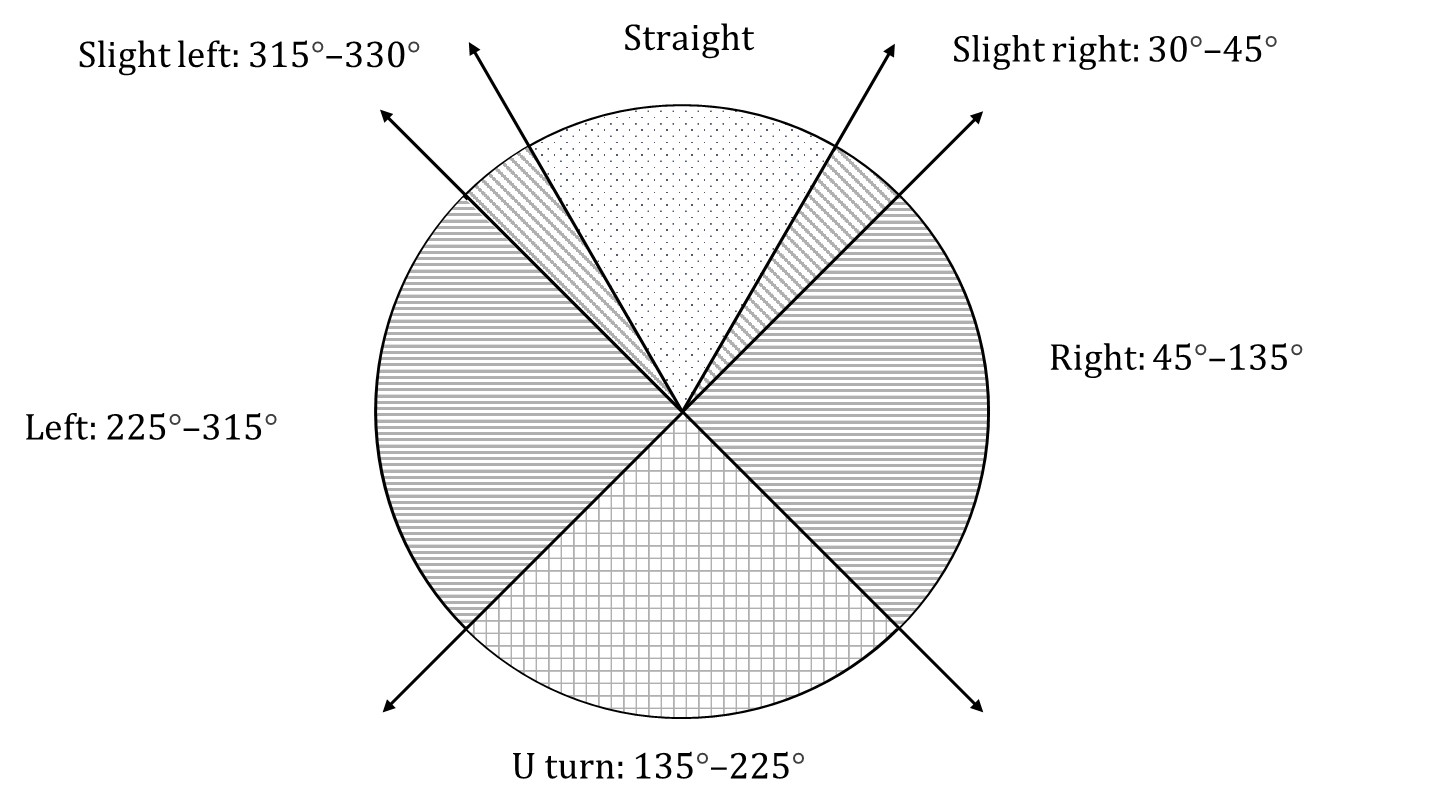
\includegraphics[width=1.0\textwidth]{fig_turns_definition.jpg}
    \caption{Angular definition of turns in the model.}\label{fig:turns_definition}
\end{figure*}

\subsection{Travel Time Prediction}

Our travel time prediction model has two steps. First, we calculate \enquote{naïve travel times} across a set of trips using open data and open-source software. Second, we train a random forest regression model to predict the Google \enquote{gold standard} travel times from our \enquote{naïve travel times} plus a set of covariates. This subsection details this process.

To calculate naïve travel times, we solve each OD pair's shortest path using Dijkstra's algorithm to minimize edge traversal time at the speed limit. Then we count the number of traffic control elements (including traffic signals, pedestrian crossings, give ways, and mini roundabouts) and turns (i.e., left, slight left, right, slight right, and u-turn), as shown in Figure~\ref{fig:turns_definition}, along each OD pair's route.

Then we train a random forest regression model to predict a route's Google travel time from  the naïve travel time plus the count of each type of traffic control element and turn encountered along the naïve shortest path. We also tested other algorithms, including ordinary least squares, gradient boosting regression, AdaBoost regression, and decision tree regression, but settled on random forest regression as its ensemble accuracy substantially outperforms the others.

We divide our OD pairs into a standard 80/20 training/test split, then tune the hyperparameters through a randomized grid search with 5-fold cross-validation by calculating their mean absolute error (MAE), defined in Equation~\ref{eq:mae}:

\begin{equation}
\label{eq:mae}
\text{MAE} = \frac{\sum^{n}_{i=1} \left|{t_i - \hat{t_i}}\right|}{n}
\end{equation}

where $n$ is the total number of trips, $t_i$ is trip $i$'s observed travel time, and $\hat{t_i}$ is trip $i$'s predicted travel time.

\subsection{Validation}

We validate our out-of-sample predictions against the \enquote{gold standard} Google travel times using five measures. First, we calculate the MAPE, following Equation~\ref{eq:mape}. Second, we calculate the MAE, following Equation~\ref{eq:mae}, to measure the average absolute difference in seconds between our prediction and the reference Google value. Third, we perform difference-in-means ($\delta$) $t$-tests to determine whether our predicted travel times are statistically significantly different (at the $p<=0.05$ significance level) from the reference Google values. Despite the large sample size, we expect insignificant $t$-statistics if the predicted travel times' distribution approximates the Google travel times' distribution. Fourth, we calculate the standard $R^2$ to measure our model's success in explaining travel time variation. Fifth and finally, we calculate the average of the pairwise ratios (APR) of our predicted travel time and the Google travel time to measure the average over- or under-prediction of the trips' travel times, as defined in Equation~\ref{eq:apr}:

\begin{equation}
\label{eq:apr}
\text{APR} = \frac{\sum^{n}_{i=1}\frac{t_i}{\hat{t_i}}}{n}
\end{equation}

where $n$ is the total trip count, $t_i$ is trip $i$'s Google travel time, and $\hat{t_i}$ is our predicted travel time for trip $i$.

\section{Results}

\subsection{Optimized Hyperparameters}

Our final optimized model hyperparameterization uses 600 decision trees, random sampling with replacement in each decision tree, a maximum decision tree depth of 10, a non-limited maximum number of input explanatory features, a requirement of at least two samples to split at a decision node and one sample at a leaf node, and equal sample weighting. Finally, we check our trained model for overfitting by conducting 5-fold cross-validation across the whole sample using tuned hyperparameters: the resulting five MAE values (75.3, 74.5, 73.5, 73.3, 74.7) are all similar to each other, which indicates no overfitting problem as the hyperparameters are not overly specific to the training set.

\subsection{Model Performance and Validation}

Table~\ref{tab:validation_results} details our travel time prediction model's out-of-sample improvement over the initial naïve travel time calculation. Our model achieves a MAPE of 8.4\%, in line with the approximately 10\% MAPEs seen in the state-of-the-art travel time prediction literature, but without their extensive and expensive input data requirements. In comparison, our initial naïve travel time calculation yields a much worse MAPE of 21.1\%. Whereas the naïve travel time calculation's MAE is 183.5 seconds from the Google travel time, our predicted travel times' MAE is just 75.2 seconds---an improvement by a factor of 2.4.

\begin{table*}[tb!]
    \centering
    \caption{Results of out-of-sample (testing set) prediction of (1) our prediction model and (2) the initial naïve travel time calculation, validated against the corresponding Google travel times. The five validation measures are (1) MAPE, (2) MAE, (3) difference-in-means ($\delta$) and corresponding $t$-test $p$-value, (4) APR, and (5) $R^2$. See methods for definitions.}\label{tab:validation_results}
    \begin{tabular}{lrr}
        \toprule
                                      & Prediction model & Naïve calculation \\
        \midrule
        MAPE (\%)                     &             8.43 &             21.13 \\
        MAE (seconds)                 &            75.23 &            183.55 \\
        $\delta$ (seconds)            &             0.38 &           -182.71 \\
        $p$-value                     &             0.75 &             <0.01 \\
        APR                           &             1.01 &              0.79 \\
        $R^2$                         &             0.93 &              0.74 \\
        \midrule
        $n$                           &           8,272 &            8,272 \\
        \bottomrule
    \end{tabular}
\end{table*}

The $t$-test reveals significant differences between the initial naïve travel time calculations and the Google travel times: the $\delta$ of -182.7 seconds corresponds to $p<0.01$. In other words, the naïve travel time under-predicts Google by over 3 minutes. However, the $t$-test reveals insignificant differences between our model's out-of-sample predictions and the Google travel times: the $\delta$ of 0.4 seconds corresponds to a $p$ value of 0.75. That is, our prediction model over-predicts by less than half a second on average, which is statistically insignificantly different from zero. If we compare the aforementioned MAEs to these differences-in-means, we can see that the initial naïve travel time calculations significantly and consistently under-predict travel time, but our prediction model shows no such directional bias: its random error balances out between (smaller absolute) over-and under-prediction.

The APR offers another lens on this finding. On average across the OD pairs, the initial naïve travel time calculation under-predicts Google travel time by 21\%, but our prediction model over-predicts it by just 1\%. Our model also explains more of the variation in travel time: its $R^2$ of 0.93 is substantially higher than the 0.74 $R^2$ of the initial naïve travel time calculation. In summary, each of our five validation measures demonstrates that our prediction model drastically improves on naïve travel time calculations---without needing extensive, expensive input data or advanced deep learning software---and offers travel time predictions much closer to those of Google's \enquote{gold standard} predictions.

\section{Discussion}

Re-state the problem. This study set out to investigate if a middle-ground travel time prediction model was possible. It identified three criteria for success: (1) it should use free software and data and avoid bespoke sensor data collection; (2) it should be easy and accessible to use; (3) it should offer better accuracy than naïve predictions (e.g., minimizing Euclidean distance, network distance, street edge traversal time) and better spatial resolution than zone-to-zone travel times.

Our results show that our proposed method satisfies these criteria to offer an important middle-ground contribution. First, it relies only on open-source Python software, OpenStreetMap data, and a small free amount of Google travel time training data. Second, our model is easy to use: it does not require a complex computing environment suited for deep learning's extensive data and processing requirements. Rather, our model uses out-of-the-box tools that can be set up in seconds on a standard consumer-grade computer by anyone familiar with Python, the world's most popular programming language. Third, our model is accurate: its MAPE (8.4\%) is much lower than that of the naïve model and in line with state-of-the-art models (\textasciitilde3--17\%) with extensive data and computing requirements.

This middle ground is not necessarily for computer scientists, high-end labs with top-of-the-line computing hardware, or well-resourced agencies with extensive data budgets. Rather, it empowers the scholars and practitioners who need it the most---those working on the frontlines of urban planning and policymaking. These scholars and practitioners rely on simple but inaccurate routing models---such as minimizing Euclidean distance, network distance, or edge traversal time---when they lack the technical expertise, computing equipment, or extensive data needed to implement the literature's cutting-edge models. However, this study demonstrated how these naïve methods systematically under-predict real-world travel times. Our model addresses this problem by incorporating sparse open data on traffic control elements and turns into the prediction and achieves an accuracy in line with state-of-the-art methods---but without their data needs or computing requirements. In other words, our model does not replace the state-of-the-art methods for those with extensive resources available to implement them, but rather offers far more accurate predictions for urban planners who would otherwise fall back on simpler naïve models. Inaccurate travel times skew empirical understandings and mislead planning interventions. Our model represents an important contribution for urban planning scholarship and evidence-based practitioner interventions.

As demonstrated, this model supports high-resolution point-to-point travel time predictions across a large metropolitan area. Our implementation focused on Los Angeles but is not inherently tied to it, and future work should emphasize its generalizability in cities with potentially sparser or lower-quality open data. We trained this model as a proof-of-concept for minimally-congested times of day, but the same concept can be extended with similar training data for any other time of day. Future research should also expand the kinds of training and validation data. Although used by billions of people around the world as the public's \enquote{best available} source of travel time prediction, Google travel time remains a black box based on users' GPS data. Future work can use other empirical travel time data to further train and validate the model.

\section{Conclusion}

Travel time prediction is central to questions of urban accessibility, mode and route choice, and individuals' location decisions. True congested travel time vary drastically throughout the day and require large volumes of real-time or proprietary data, as well as complex algorithms, to model. These technical challenges and costs present a hurdle for many urban planners, who often turn to simpler models with lower and often free data and computing requirements. The traditional naïve methods are easy to implement, but produce inaccurate predictions.

This article introduced a middle-ground method to simply but accurately predict minimally-congested travel time using free data. It improves on traditional, common, naïve predictions by training on a small one-off collection of free but proprietary high-quality Google data on travel times. Also of note is the sparseness of our open data: OpenStreetMap contains little information on traffic controls, as only around 28\% of the intersections in the study area have traffic control information. Even so, our prediction model using random forest regression still predicts Google travel times with high accuracy. This offers planning practitioners and scholars a better method to predict travel times for free with much better accuracy than traditional naïve methods offered.

\section*{Acknowledgments}

The authors wish to thank Youngseo Kweon and Jaehyun Ha for additional research assistance.

% print the footnotes as endnotes, if any exist
\IfFileExists{\jobname.ent}{\theendnotes}{}

% print the bibliography
\setlength{\bibsep}{0.00cm plus 0.05cm} % no space between items
\bibliographystyle{apalike}
\bibliography{references}

\end{document}
